%!TEX root = main.tex

\section{Index Reduction Algorithm}

\begin{frame}{Index Reduction Algorithm}{The Basic Concept}
  The index reduction algorithm is based on the following three steps \dots
  \begin{columns}
    \begin{column}[c]{0.2\textwidth}
      \flushright
      \vspace{-2.5em}%
      \uncover<4->{\begin{tikzpicture}[overlay, remember picture]
        \draw[fg_sl_color, thick, -stealth] (0.5,-1.95) -- (0.0,-1.95) -- (0.0,1.95) -- (0.5,1.95);
        \node[text width=0.75\textwidth, align=center] at (-1.0,0.0) {If $\mE$ is singular};
        %\draw[fg_sl_color, thick, -stealth] (-1.0,-0.5) -- (-1.0,-2.75);
      \end{tikzpicture}}
    \end{column}
    \begin{column}[c]{0.85\textwidth}
      \begin{enumerate}[<+->]
        \item Let us consider a generic system of \acp{DAE} of the form
        \begin{equation*}
          \mF = \mA \, \mxp - \mb = \m{0} \text{.}
        \end{equation*}
        \item We want to separate the system into \textbf{differential} and \textbf{algebraic} equations and express the system in \textbf{semi-explicit} form
        \begin{equation*}
          \left\{\!\!\!\begin{array}{r@{~}c@{~}l}
            \mE \, \mxp &=& \mg \\
            \m{0}\phantom{\prime} &=& \ma
          \end{array}\!\!\!\right. \text{.}
        \end{equation*}
        \item The index of the system is reduced by differentiating the algebraic equations $\ma = \m{0}$.
      \end{enumerate}
    \end{column}
  \end{columns}
  \vspace{0.75em}
  \uncover<5->{\dots and it can be applied until a \acs{ODE} system with invariants is obtained.}
\end{frame}

\begin{frame}{Index Reduction Algorithm}{Separation of Differential and Algebraic Equations}
  \begin{itemize}
    \item Let us consider a generic system of \acp{DAE} of the form
    \begin{equation*}
      \mF = \mA \, \mxp - \mb = \m{0} \text{.}
    \end{equation*}
    %
    \item The differential equations can be separated from the algebraic ones by exploiting the kernel $\mK$ and its orthogonal complement $\mN$ of $\mE^\top$ such that
    \begin{equation*}
      \left\{\!\!\!\begin{array}{r@{~}c@{~}l}
        \mE \, \mxp &=& \mg \\
        \m{0}\phantom{\prime} &=& \ma
      \end{array}\right.
      \qquad \text{where} \qquad
      \begin{array}{r@{~}c@{~}l}
        \mE &=& \mN \, \mA \text{,} \\
        \mg &=& \mN \, \mb \text{,} \\
        \ma &=& \mK \, \mb \text{.}
      \end{array}
    \end{equation*}

    \begin{bbox}[Kernel Computation]
      To calculate the kernel $\mK$ and its orthogonal complement $\mN$ of $\mE^\top$ we use \ac{LU} or \ac{FFLU} matrix factorizations.
    \end{bbox}
  \end{itemize}
\end{frame}

\begin{frame}{Index Reduction Algorithm}{Differentiation of Algebraic Equations}
  \begin{itemize}
    \item We can differentiate the algebraic equations $\ma$
    \begin{equation*}
      \dfrac{\mathrm{d}}{\mathrm{d}t} \ma = \mAd \, \mxp - \mgd \text{.}
    \end{equation*}
    %
    \item The new system of \acp{DAE} with reduced index takes the form
    %
    \begin{align*}
      \mF = \mA \, \mxp - \mb = \m{0}
      \hspace{0.75em} \text{with} \hspace{0.75em}
      \mA = \begin{bmatrix} \mE \\ \mAd \end{bmatrix}
      \hspace{0.75em} \text{and} \hspace{0.75em}
      \mb = \begin{bmatrix} \mg \\ \mgd \end{bmatrix} \text{.}
    \end{align*}
    %
    \item The differential index of the system has been reduced by one
  \end{itemize}
  %
  \begin{bbox}[A Sequential Algorithm \dots]
    This algorithm is applied repeatedly until any algebraic equation $\mA$ is left, or equivalently until the matrix $\mE$ is non-singular.
  \end{bbox}
\end{frame}

\begin{frame}{Index Reduction Algorithm}{Including Veiling Variables}
  The algorithm can be extended to include \acl*{LEM} \dots
  \begin{itemize}
    \item the veiling variables are stored in the vector $\mv$;
    \item the matrices $\mE$ and $\mA$ will be also functions of the veil variable $\mv$;
    \item If the veiling variables do not depend on the state variables derivatives, they just add an evaluation layer to the algorithm.
  \end{itemize}
  %
  \vspace{0.5em}
  %
  \centering{\begin{tikzpicture}
    \node at (0,0) {$\mx$};
    \node at (1.5,1.5) {$\mv$};
    \node at (1.5,1.85) {Additional evaluation layer};
    \node at (3,0) {$\begin{array}{c} \mEv \\ \mAv \\ \mhv \end{array}$};
    \node at (1.5,-1.5) {$\mxp$};
    \draw[fg_sl_color, thick, -stealth] (0.35,0.0) -- (2.05,0.0);
    \draw[fg_sl_color, thick, stealth-] (0.75,1.5) -| (0.0,0.35);
    \draw[fg_sl_color, thick, stealth-] (0.0,-0.35) |- (1.05,-1.5);
    \draw[fg_sl_color, thick, stealth-] (3.0,0.75) |- (2.25,1.5);
    \draw[fg_sl_color, thick, stealth-] (3.0,-0.75) |- (1.85,-1.5);
    \draw[fg_sl_color, dashed, line width=1.0pt] (-0.6,2.2) rectangle (3.6,1.1);
  \end{tikzpicture}}
\end{frame}

\begin{frame}{Index Reduction Algorithm}{Algorithm Flowchart}
  \centering
  \begin{tikzpicture}[overlay]
    \node at (0,0) {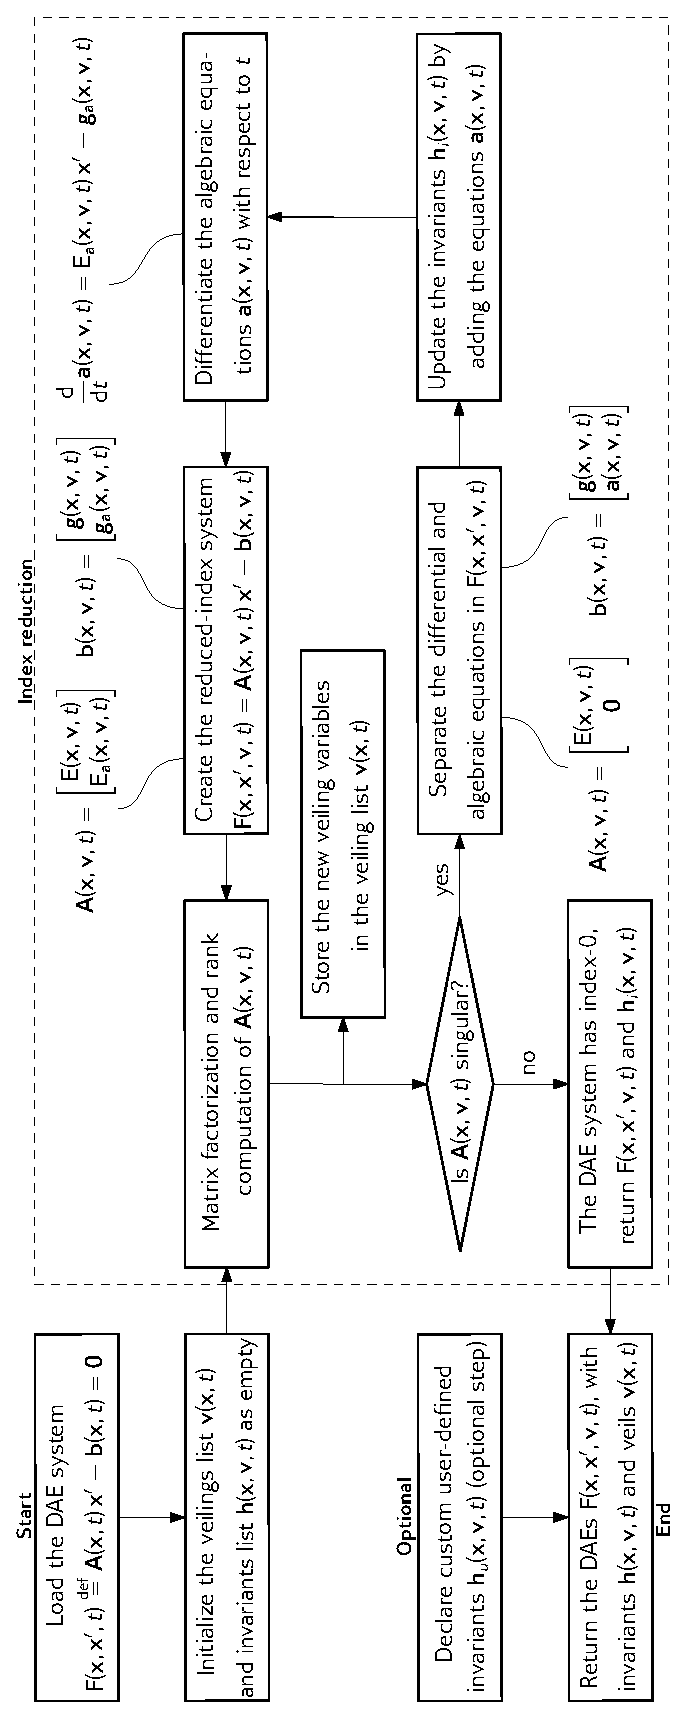
\includegraphics[angle=270, width=1.0\textwidth]{dae_flowchart_veil}};
    \only<1>{\draw[fg_sl_color, line width=1.0pt] (-7.2,  2.9) rectangle (-3.7,  0.4);} % Initialization
    \only<2>{\draw[fg_sl_color, line width=1.0pt] (-3.7,  2.9) rectangle ( 7.2, -2.9);} % Index Reduction
    \only<3>{\draw[fg_sl_color, dashed, line width=1.0pt] (-7.2, -0.3) rectangle (-3.7, -1.6);} % Optional step
    \only<4>{\draw[fg_sl_color, line width=1.0pt] (-7.2, -1.6) rectangle (-3.7, -2.9);} % Finalization
  \end{tikzpicture}
\end{frame}

\begin{frame}{Index Reduction Algorithm}{The Reduced \ac{DAE} System}
  The index-reduced system of \acp{DAE} takes the form \dots
  \begin{itemize}[<+->]
    \item A \textbf{differential part}, which can be expressed as
    %
    \begin{equation*}
      \begin{array}{ccl}
          \m{F}(\mx, \mx^\prime, \m{v}, t) = \m{0} & \hspace{0.5cm} & \text{implicit  system class,} \\
          \m{A}(\mx, \m{v}, t) \, \mx^\prime = \m{b}(\mx, \m{v}, t) & \hspace{0.5cm} & \text{semi-explicit system class,} \\
          \mx^\prime = \m{f}(\mx, \m{v}, t) & \hspace{0.5cm} & \text{explicit system class.}
      \end{array}
    \end{equation*}
    %
    \item The \textbf{invariants}, arising from the index reduction
    %
    \begin{equation*}
      \m{h}(\mx, \m{v}, t) = \begin{bmatrix}
          \mhiv \\
          \mhuv
      \end{bmatrix} = \m{0} \hspace{0.5cm} \begin{array}{l}
        \text{hidden constraints,} \\
        \text{optional user-defined invariants.}
    \end{array}
    \end{equation*}
    %
    \item The \textbf{veiling variables}, used to limit expression swell
    %
    \begin{equation*}
        \m{v}(\mx, t) = \msmall{\begin{bmatrix}
            v_{1}(\mx, t) \\
            v_{2}(v_{1}, \mx, t) \\
            \vdots \\
            v_{n}(v_{1}, \dots, v_{n-1}, \mx, t)
        \end{bmatrix}} \, \text{.}
    \end{equation*}
  \end{itemize}
\end{frame}

% That's all Folks!